[IKKE NOGEN BESTEMT ORDEN ENDNU]
[TABELLER ER IKKE BLIVE INDLEJRET ENDNU]
Dette afsnit kommer til at handle om hvordan man kan beskrive dette projekts problemområde, en husholdnings administration af pligter og børne økonomi, i form af klasser og hændelser. Klasserne er overordnede repræsentationer af objekter, som en forælder eller en pligt, hvor hændelser er de ting som en klasse kan forårsage eller blive påvirket af. I dette problemområde vil klasserne være sådan noget som en forældre, en pligt, et barn osv., mens en hændelse kunne være at en forælder opretter en ny pligt, og derefter en anden hændelse hvor et barn optager pligten. En hændelsestabel for dette problemområde kan blive set i figur [REF].

[TABEL]

Tabellen kan blive udvidet yderligere, ved at inkludere en klasse som konto eller graf, som sagtens kan blive inkluderet under en de andre mere fremtrædende klasser eller hændelser. En konto er inkluderet i barn klassen, og graf klassen er dels inkluderet i både barn og forældre klassen, samt ’se statistik’ hændelsen. En ‘Anmodning’ er i denne sammenhæng en besked et barn sender til sin forælder om, at det har fuldført sin tilskrevet pligt, og ønsker den behandlet.

Herefter kan klasserne blive opsat i et klassediagram, med henhold til deres indbyrdes relationer. Dette klassediagram kan blive set i figur [REF]. Klassehierarkier bliver vist indkapslet i kasser, samt pile fra underklasser til superklasser. Horisontale streger vise associering, som model og forælder, hvor lommepenge modellen går ind og påvirker på hvad forældrene gør i forhold til pligter og udbetalinger. En klasse som tilhører en anden klasse bliver vist lignende den for klassehierarkiet, men med en rombe i stedet for en pil. Ligeledes angiver tallene mængden af hver klasse til en anden klasse. For eksempel så er en pligt altid kun forbundet til den forælder som lavet den, mens en forælder sagtens kan lave adskillige pligter.

\begin{figure}[htb]
\centering
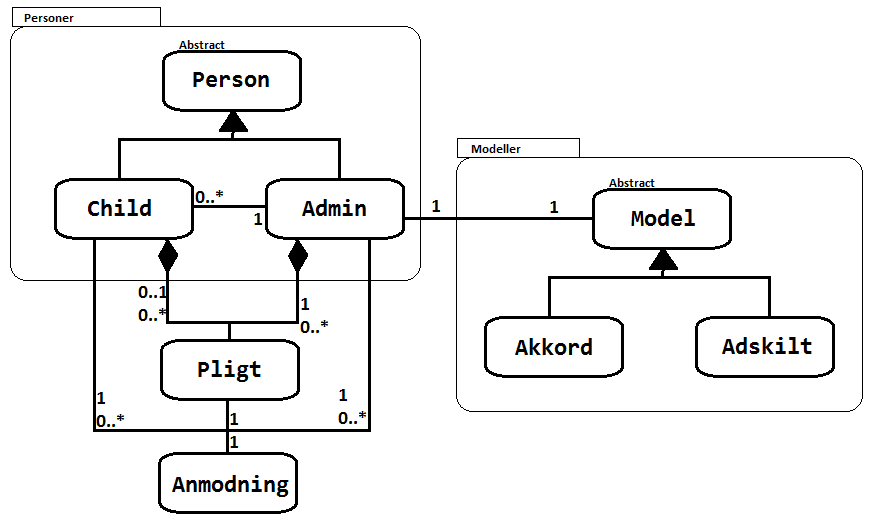
\includegraphics[width=0.8\textwidth]{Billeder/KlasseDiagram.png}
\caption{KlasseDiagram}
\label{KlasseDiagram}
\end{figure}

Diagrammet kan blive skrevet meget mere indviklet, hvis man gør op for alle mulige relationer mellem klasserne. En anmodning kunne ligeså vel sat i forbindelse med en pligt, og man kunne begynde lave klasser for pligt kvitteringer, eller en pil mellem barn og pligt for også at vise en mulige liste af allerede udførte pligter, som bliver beholdt til arkivering og statistik. Dette skulle gerne give et ove